\setchapterpreamble[u]{\margintoc}
\chapter{Ecuaciones de Klein-Gordon y de Dirac}
\labch{Part}

\begin{center}
  \large Todo esto lo he sacado de \cite{Dobdado}
\end{center}
\section{Ecuación de Klein Gordon}
Recordemos que bajo el sistema natural de unidades, el Hamiltoniano de una partícula relativista es simplemente $H=\sqrt{\vec{p}^{2}+m^{2}}$, con $c=1$. La ecuación de Klein-Gordon busca una descripción relativista de la ecuación de Schrödinger:
$$
\sqrt{\vec{p}^{2}+m^{2}} \psi(\vec{x}, t)=i \frac{\partial}{\partial t} \psi
$$

Volviéndola a aplicar para quitar las raíces cuadradas:
$$
\begin{gathered}
\left(\vec{p}^{2}+m^{2}\right) \psi=-\frac{\partial^{2} \psi}{\partial t^{2}} \\
\left(\frac{\partial^{2}}{\partial t^{2}}-\nabla^{2}+m^{2}\right) \psi(\vec{x}, t)=0
\end{gathered}
$$

Está es la ecuación de Klein-Gordon, que es invariante relativista. A continuación, un breve inciso explicando como obtener los cuadrivectores y sus operadores.

Recordemos la definición de cuadrivector contravariante $V^{\mu}=\left(V^{0}, \vec{V}\right)$. Se definen las componentes covariantes a partir del tensor métrico:
$$
g_{\mu \nu}=\left(\begin{array}{llll}
1 & & & \\
& -1 & & \\
& & -1 & \\
& & & -1
\end{array}\right)
$$

Si tengo dos cuadrivectores, $A^{\mu}=\left(A^{0}, \vec{A}\right)$ y $B^{\mu}=\left(B^{0}, \vec{B}\right)$, podemos definir el producto escalar (en sentido Minkowski ${ }^{1.3}$ ) como:
$$
A \cdot B=A^{\mu} B^{\nu} G_{\mu \nu}=A^{0} B^{0}-\vec{A} \cdot \vec{B}
$$

Así mismo, definimos las componentes covariantes se obtienen a partir de la métrica: $V_{\mu}=g_{\mu \nu} V^{\nu}=\left(V_{0},-\vec{V}\right)$. De esta manera:
$$
V^{2}=V^{\mu} V^{\nu} g_{\mu \nu}=V^{\mu} V_{\mu}=V^{0^{2}}-\vec{V}^{2}
$$

Esta norma, en el espacio de Minkowski, no está definida positiva (en función del género: tiempo, luz, espacio).

\footnotetext{
${ }^{1.3} \mathrm{El}$ producto escalar en sentido Minkowski es invariante Lorentz.
}

Con:
$$
\begin{aligned}
\rho & =\frac{i}{2 m}\left(\psi^{*} \partial_{t} \psi-\psi \partial_{t} \psi^{*}\right) \\
\vec{j} & =\frac{-i}{2 m}\left(\psi^{*} \vec{\nabla} \psi-\psi \vec{\nabla} \psi^{*}\right)
\end{aligned}
$$

Si hacemos el cuadrigradiente de la densidad de corriente:
$\partial_{\mu} J^{\mu}=\frac{i}{2 m}\left(\partial_{\mu} \psi^{*} \partial^{\mu} \psi+\psi^{*} \square \psi-\partial_{\mu} \psi \partial^{\mu} \psi^{*}-\psi \square \psi^{*}\right)=0 \rightarrow \partial_{\mu} J^{\mu}=\frac{\partial \rho}{\partial t}+\vec{\nabla} \cdot \vec{j}=0$
Esto último nos verifica que cumple la ecuación de continuidad.
\section{Ecuación de Klein-Gordon en presencia de campos electromagnéticos}
En el sistema de unidades Heaviside-Lorentz las ecuaciones de Maxwell verifican:
$$
\begin{array}{cc}
\vec{\nabla} \cdot \vec{B}=0 ; & \vec{\nabla} \times \vec{E}+\frac{1}{c} \frac{\partial \vec{B}}{\partial t}=0 \\
\vec{\nabla} \cdot \vec{E}=0 ; & \vec{\nabla} \times \vec{B}=\frac{1}{c} \vec{j}+\frac{1}{c} \frac{\partial \vec{E}}{\partial t} \\
\vec{E}, \vec{B} ; & \vec{B}=\vec{\nabla} \times \vec{A} \\
\phi, \vec{A} ; & \vec{E}=-\vec{\nabla} \cdot \phi-\frac{\partial \vec{A}}{\partial t}
\end{array}
$$

El objetivo de estas unidades es que las ecuaciones de Maxwell sean lo más sencillo posible. Si además imponemos sistema natural:
$$
\begin{array}{ll}
\vec{\nabla} \cdot \vec{B}=0 ; & \vec{\nabla} \times \vec{E}+\frac{\partial \vec{B}}{\partial t}=0 \\
\vec{\nabla} \cdot \vec{E}=\rho ; & \vec{\nabla} \times \vec{B}=\vec{j}+\frac{\partial \vec{E}}{\partial t}
\end{array}
$$

El Lagrangiano de una partícula interaccionando con campo eléctrico y magnético es:
$$
\begin{equation*}
\mathcal{L}=-m \sqrt{1-v^{2}}+q \vec{v} \cdot \vec{A}-q \phi=\mathcal{L}(\vec{x}, \vec{v}) \tag{1.6}
\end{equation*}
$$

Con $-m \sqrt{1-v^{2}}$ el término de partícula libre, $q \vec{v} \cdot \vec{A}$ el término de interacción magnética $\mathrm{y}-q \phi$ el correspondiente a la interacción eléctrica.

El Hamiltoniano está definido en función de $\vec{x}$ y de $\vec{\Pi}$, con $\vec{\Pi}=\frac{\partial \mathcal{L}}{\partial \vec{v}}=\vec{\rho}+q \vec{A}$, el momento canónicamente conjugado; que es distinto a la cantidad de movimiento, $\vec{p}=m \gamma \vec{v}$.

El cuadrivector $p^{\mu}=(E, \vec{p})$ en representación de posiciones $(|x\rangle)$ :
$$
P^{\mu}=\left(i \frac{\partial}{\partial t},-i \vec{\nabla}\right) \rightarrow P^{\mu}=i \partial^{\mu}
$$

De aquí, a partir de la expresión para obtener un Hamilotniano a partir del Lagrangiano de un sistema:
$$
H\left(q_{i}, p_{i}\right)=\sum_{i} \dot{q}_{i} p_{i}-\mathcal{L} \rightarrow H(\vec{x}, \vec{\Pi})=\vec{v} \cdot \vec{\Pi}-\mathcal{L}
$$

Obteniendo la siguiente expresión para el Hamiltoniano del sistema:
$$
\begin{equation*}
H(\vec{x}, \vec{\Pi})=\sqrt{m^{2}+(\vec{\Pi}-q \vec{A})^{2}}+q \phi \tag{1.7}
\end{equation*}
$$

Con $(\vec{\Pi}-q \vec{A})^{2}=\vec{p}^{2} ; \sqrt{m^{2}+(\vec{\Pi}-q \vec{A})^{2}}=E$, el término de la energía relativista y $q \phi$ la energía electromagnética (no contribuye el campo magnético ya que no acelerá trayectorias, solo las curva).

Comparando con las ecuaciones de una partícula, para introducir el campo electromagnético hay que hacer los siguientes cambios:
$$
\left.\begin{array}{c}
i \partial_{t} \longrightarrow i \partial_{t}-q \phi \\
-i \vec{\nabla} \longrightarrow-i \vec{\nabla}-q \vec{A}
\end{array}\right\} \partial^{\mu} \rightarrow \partial^{\mu}+i q A^{\mu} \rightarrow \partial^{\mu} \longrightarrow D^{\mu}=\partial^{\mu}+i q A^{\mu}
$$

Con $\mathcal{D}^{\mu}$ la derivada covariante. Así, la ecuación de Klein-Gordon para la interacción EM queda:
$$
\begin{gather*}
\left(\square+m^{2}\right) \psi=0 \longrightarrow\left(D_{\mu} D^{\mu}+m^{2}\right) \psi=0 \rightarrow \\
\rightarrow\left[\left(i \frac{\partial}{\partial t}-q \phi\right)^{2}-(-i \vec{\nabla}-q \vec{A})^{2}\right] \psi=m^{2} \psi \tag{1.8}
\end{gather*}
$$

Esta es la ecuación de Klein-Gordon para una partícula cargada en presencia de un campo EM.

Si ahora introducimos la carga $q$ en el cuadrivector $J^{\mu}$ :
$$
J^{\mu}=\frac{i q}{2 m}\left(\psi^{*} \partial^{\mu} \psi-\psi \partial^{\mu} \psi^{*}=(\rho, \vec{j})^{1.4}\right.
$$

Que, nuevamente, cumple la ecuación de continuidad.
Si $\psi \in \mathbb{R} \rightarrow \psi=\psi^{*}=J^{\mu}=0$, es decir, si la función de onda es real, representa una partícula neutra y, por tanto, una partícula cargada debe tener función de onda compleja.
\section{Ecuación de Dirac}

A continuación vamos intentar solucionar algunos de los problemas que tenía la ecuación de Klein-Gordon y para ello vamos a definir la siguiente base de estados:

\[\ket{\vec{x},s}\Rightarrow\psi_{s}=\bracket{\vec{x},s}{\psi(t)}=\psi_{s}(\vec{x},t)\]
\todo{La $s$ tiene que ver con el espín, pero no es exactamente el espín}
en donde $s=s_{1},s_{2},\dots,s_{m}$ y $\Psi= \begin{bmatrix}
    \psi_{1}\\
    \psi_{2} \\
    \vdots \\
    \psi_{m}
\end{bmatrix}$

A continuación definimos un nuevo hamiltoniano llamado \textit{Hmailtoniano de Dirac} el cual tiene la forma 

\[H_{D}=\vec{\alpha}\vec{\mathscr{P}}+\beta\]
en donde $\alpha,\beta$ son matrices de $m\times n$ dimensiones. 

Aplicando este Hamiltoniano a la ecuacion de Shrödinger obtenemos 
\begin{DispWithArrows}[format=ll, displaystyle]
  i \partial_t\Psi = H_D \Psi \Rightarrow & H_D \Psi=E\Psi \\
  \Rightarrow & E\Psi=H_D\Psi \\
  \Rightarrow & (E-H_D)\Psi=0 \\
  \Rightarrow & (E-\vec{\alpha}\vec{\mathscr{P}}-\beta)\Psi=0
  \label{eq:D}
\end{DispWithArrows}

La ecuación de Klein-Gordon es correcta por lo que se tiene que satisfacer que $E^{2}=p^{2}+m^{2}$ de forma que  

\begin{DispWithArrows}[format=l, displaystyle]
  (E+\vec{\alpha}\vec{\mathscr{P}}+\beta)(E-\vec{\alpha}\vec{\mathscr{P}}-\beta)\Psi=0 \Rightarrow  (E^2-(\vec{\alpha}\vec{\mathscr{P}}+\beta)^2)\Psi=0 \\
  \Rightarrow  (E^2-\alpha_i\alpha_jP^iP^j-m\alpha_i\beta P^i-m\beta\alpha_iP^i-m^2\beta^2)\Psi=0 \Arrow{$i=j$} \\
  \Rightarrow  (E^2-\sum) \\
  \Rightarrow  
  \label{eq:}
\end{DispWithArrows}
\todo{Para acortar vamos a usar el convenio de Einstein de inidces repetidos, en este caso esto es $
  \alpha_{i}\alpha_{j}P^{i}P^{j}= \sum_{ij}\alpha_{i}\alpha_{j}P_{i}P_{j}$}

  De esta última ecuación podemos obtener los coeficientes de las matrices $\alpha$ y $\beta$ que cumplen la ecuación de K-G, los cuales deben cumplir las siguientes propiedades:

  \begin{itemize}
    \item $\alpha_{i}^{2}=\beta^{2}_{i}=\mathcal{I}$
    \item $\acomm{\alpha_{}}{\alpha_{j}}=0~ \forall i \neq j$
    \item $\acomm{\alpha_{i}}{\beta}=0$
    \item $\alpha^{i}=(\alpha^{i})^{\dagger}$ y $\beta^{i}=(\beta^{i})^{\dagger}$
  \end{itemize}

  De esta forma la ecuación de Dirac por componentes \marginnote[-2.2cm]{
    \begin{kaobox}[frametitle=Recuerda]
      $\Psi= \begin{bmatrix}
        \psi_{1}\\
        \psi_{2} \\
        \vdots \\
        \psi_{m}
    \end{bmatrix}$
  \end{kaobox}
  } queda con la forma

  \begin{DispWithArrows}[format=c, displaystyle]
    i(\partial_t +i\vec{\alpha}\cdot\vec{\nabla}- \beta m)\psi_s=0
    \label{eq:dcomp}
  \end{DispWithArrows}

A continuación vamos a definir lo que se denominan \textit{Matrices de Dirac}, las cuales se definen como

\[\gamma^{0}=\beta\qquad\gamma^{i}=\beta\alpha^{i}\]

con $\alpha^{i}=\alpha_{i}$. Podemos expresarlas en forma indicial, \textbf{pero sin ser un cuadrivector}, con la forma $\gamma^\mu=(\gamma^{0},\gamma^{i})$. 

Podemos expresar las condiciones de los coeficientes $\beta$ y $\alpha$ con estas matrices de forma mucho más abrebiada como 
\[\acomm{\gamma^{\mu}}{\gamma^{\nu}}=2g^{\mu\nu}\]

Se puede demostrar que estas condiciones solo se satisfacen para matrices con dimensiones pares, pero además se puede demostrar que la dimensión mínima que han de tener para que se cumplan es 4, por lo que solo se cumplen para aquellas con $n\geq4$ siendo $n$ el número de componentes del espinor de Dirac $\Psi$. 

Podemos escribir la ecuación \ref{eq:D} con las matrices $\gamma$ de la forma 

\[(i\gamma^{\mu}\partial_{\mu}+m)\Psi=0\]

Esta ecuación no es covariante ya que $\gamma^{\mu}$ no es un cuadrivector ni $\Psi$ es un escalar (es decir, función $\Psi(x)$); pero si es un invariante relativista. 

A continuación veamos la forma de estas matrices $\gamma$  en diferentes representaciones:
\begin{itemize}
  \item Representación de Dirac
  \[\gamma^{0}=\begin{pmatrix}
      \mathbb{I} & 0 \\
      0 & \mathbb{I} 
  \end{pmatrix}\qquad \vec{\gamma}= \begin{pmatrix}
      0 & \vec{\sigma} \\
      \vec{\sigma} & 0 
  \end{pmatrix}\]
  \item Representación de Weyl
  \[\gamma^{0}=\begin{pmatrix}
      0 & \mathbb{I} \\
      \mathbb{I} & 0 
  \end{pmatrix}\qquad \vec{\gamma}= \begin{pmatrix}
      0 & \vec{\sigma} \\
      \vec{\sigma} & 0 
  \end{pmatrix}\]
\end{itemize}
Como podemos ver entre una representación y otra solo cambia $\gamma^{0}$, pero el cambio es importante ya que si \textbf{cambiamos las matrices, cambiamos el significado físico de las componentes del espinor de Dirac}.

Además, podemos reconocer $\vec{\sigma}$ como las matrices sigma de Pauli, las cuales siguen la siguiente regla de conmutación y anticonmutación:
\[\sigma^{i}\sigma^{j}=\delta^{ij}+i\varepsilon_{ijk}\sigma^{k}\left\{\begin{align}
  \comm{\sigma^{i}}{\sigma^{j}}=2i\varepsilon_{ijk}\sigma^{k} \\
  \acomm{\sigma^{i}}{\sigma^{j}}=2\delta_{ij} 
\end{align}\right.\]
\subsection{Partículas cargadas en un campo electromagnético}
En electrodinámica clásica, vimos que el Lagrangiano de un sistema relativista es: $\mathcal{L}=-\frac{1}{4} F_{\mu \nu} F^{\mu \nu}$. Ahora bien, en el sistema de Maxwell-Dirac:
$$
\mathcal{L}=-\frac{1}{4} F_{\mu \nu} F^{\mu \nu}+\bar{\psi}(i \not D-m) \psi
$$

Con $F_{\mu \nu}=\partial_{\mu} A_{\nu}-\partial_{\nu} A_{\mu}$ el tensor electromagnético y $D_{\mu}=\partial_{\mu}+i q A_{\mu}$. Quedando el Lagrangiano para un sistema de una partícula sometida a un campo EM:
$$
\mathcal{L}=-\frac{1}{4} F_{\mu \nu} F^{\mu \nu}+\bar{\psi}(i \not D-m) \psi-J_{\mu} A^{\mu}
$$

Con $\vec{B}$ el campo magnético $\rightarrow \vec{B}=\vec{\nabla} \times \overrightarrow{\vec{A}}$ y $\vec{S}=\frac{\vec{\sigma}}{2}$.
En su momento Pauli definió $\varepsilon^{\prime}=\left[\begin{array}{l}\varepsilon_{+}^{\prime} \\ \varepsilon_{-}^{\prime}\end{array}\right]$
Con $\varepsilon_{+}^{\prime}$ la componente del espín hacía arriba y $\varepsilon_{-}^{\prime}$ la componente del espín hacia abajo. Además se sabía que las partículas con espín $\vec{S}$ tiene asociado un momento magnético asociado $\vec{M}_{S}$.
$$
\begin{equation*}
i \frac{\partial \varepsilon^{\prime}}{\partial t}=\left[\frac{1}{2 m}(-i \vec{\nabla}-q \vec{A})^{2}+q \phi-\vec{M}_{S} \vec{B}\right] \varepsilon^{\prime} \tag{1.15}
\end{equation*}
$$

Esta es la ecuación de Pauli, con la parte dentro del corchete el Hamiltoniano de partícula espín $\frac{1}{2}$ interactuando con un campo electromagnético no relativista.

Se definió: $\vec{M}_{S}=g \frac{q}{2 m} \vec{S}$, con $g$ el ratio giromagnético.
Comparando la ecuación de Pauli con la ecuación de Dirac en el límite no relativista:
$$
i \frac{\partial \varepsilon^{\prime}}{\partial t}=\left\{\frac{1}{2 m}(-i \vec{\nabla}-q \vec{A})^{2}-\frac{q}{m} \vec{S} \cdot \vec{B}+q \phi\right\} \varepsilon^{\prime} \rightarrow g=2
$$

Si una partícula sigue la ecuación de Dirac, su razón giromagnética es 2. Para el electrón, experimentalmente se ha medido: $\frac{g_{e}}{2}=1,001159652209 \ldots$, una precisión de 11 cifras. A partir de QED, hasta $5^{\circ}$ orden de perturbaciones, el cálculo encaja con el experimental.

El radio giromagnético para el protón medido experimentalmente es: $\frac{g_{p}}{2}=2,7928 \ldots$, la ecuación de Dirac no vale para el protón. Esto se debe a que a los hadrones ( $p, n, \pi, k, \kappa, \varphi, \ldots$ ) están compuestos por quarks ( $u, d, s, c, t, b$ ). El protón está formado por uud:
$$
\left.\begin{array}{l}
q_{u}=\frac{2}{3} e \\
q_{d}=-\frac{1}{3} e
\end{array}\right\} \frac{2}{3}+\frac{2}{3}-\frac{1}{3}=1
$$

Por eso no satisface la ecuación de Dirac ya que el protón no es partícula elemental (es un sistema).

Ocurre lo mismo con el neutrón, según Pauli $\mathrm{g}=0$ (por no tener carga), pero experimentalmente: $\frac{g_{n}}{2}=-1,9130 \ldots \rightarrow$.

Por lo mismo, es un sistema compuesto por partículas cargadas que generan corrientes provocando ese momento magnético: $n \sim u d d$. La ecuación de Dirac solo se puede aplicar a partículas elementales.

Al resolver la ecuación de Dirac para el átomo de Hidrógeno:
$$
E=E_{0}+\Delta E ; \quad E_{0}=\frac{\alpha}{2 a_{0} n^{2}}, \quad n=1,2,3, \ldots
$$

Con $\alpha=\frac{e^{2}}{4 \pi \hbar c} \sim \frac{e^{2}}{4 \pi}=\frac{1}{137}$. Además: $\Delta E=-\alpha^{2} E_{0} \frac{1}{n}\left(\frac{1}{j+\frac{1}{2}}-\frac{3}{4 n}\right)$; con $\vec{j}=\vec{l}+\vec{s}$.
La ecuación de Dirac predice la estructura fina \sidenote{Estructura fina: Aproximaciones relativistas, interacción espín-órbita y término de Darwin.} del átomo de Hidrógeno. Sin embargo no predice la hiperfina ni el efecto Lamb. Según Dirac: $E_{2 S_{1 / 2}}=E_{2 P_{1 / 2}}$, experimentalmente


son distintos por el efecto Lamb.
En resumen, la ecuación de Dirac en el límite no relativista describe partículas de $\frac{1}{2}$ y explica en parte el espectro del Hidrógeno.
\section{El límite no relativista de la ecuación de Dirac}

\section{Soluciones a la ecuación de Dirac}
\begin{center}
  \large Esta sección es de \cite{peskin_schroeder_1995}
\end{center}
Para familiarizarnos con la física de la ecuación de Dirac, analicemos ahora sus soluciones de onda plana. Puesto que un campo de Dirac $\psi$ obedece a la ecuación de Klein-Gordon, sabemos inmediatamente que puede escribirse como una combinación lineal de ondas planas:

\begin{equation*}
\psi(x)=u(p) e^{-i p \cdot x}, \quad \text { en donde } p^{2}=m^{2} \tag{3.45}
\end{equation*}

\subsection{Ondas con energía positiva}
Por el momento nos concentraremos en soluciones con frecuencia positiva, es decir, $p^{0}>0$. El vector columna $u(p)$ debe obedecer a una restricción adicional, que se encuentra introduciendo (3.45) en la ecuación de Dirac:

\begin{equation*}
\left(\gamma^{\mu} p_{\mu}-m\right) u(p)=0 \tag{3.46}
\end{equation*}


Es más fácil analizar esta ecuación en el marco de reposo, donde $p=p_{0}=(m, \mathbf{0})$; la solución para $p$ general puede entonces encontrarse potenciando con $\Lambda_{\frac{1}{2}}$. En el marco de reposo, la Ec. (3.46) se convierte en
$$
\left(m \gamma^{0}-m\right) u\left(p_{0}\right)=m\left(\begin{array}{rr}
-1 & 1 \\
1 & -1
\end{array}\right) u\left(p_{0}\right)=0
$$
y las soluciones son

\begin{equation*}
u\left(p_{0}\right)=\sqrt{m}\binom{\xi}{\xi} \tag{3.47}
\end{equation*}

para cualquier espinor numérico de dos componentes $\xi$. Convencionalmente normalizamos $\xi$ de modo que $\xi^{\dagger} \xi=1$; el factor $\sqrt{m}$ se ha insertado por conveniencia futura. Podemos interpretar el espinor $\xi$ observando el generador de rotación (3.27): $\xi$ se transforma bajo rotaciones como un espinor ordinario de dos componentes del grupo de rotación, y por tanto determina la orientación del espín de la solución de Dirac de la forma habitual. Por ejemplo, cuando $\xi=\binom{1}{0}$, la partícula tiene espín hacia arriba a lo largo de la 3-dirección.



Nótese que después de aplicar la ecuación de Dirac, somos libres de elegir sólo dos de los cuatro componentes de $u(p)$. Esto es justo lo que queremos, ya que una partícula con espín $1 / 2$ sólo tiene dos estados físicos: espín arriba y espín abajo. (Por supuesto, estamos siendo un poco prematuros al hablar de partículas y espín. Demostraremos que el momento angular de espín de una partícula de Dirac es $\hbar / 2$ cuando cuantifiquemos la teoría de Dirac en la Sección 3.5; por ahora, basta con observar que hay dos soluciones posibles $u(p)$ para cualquier momento $p$). Ahora que tenemos la forma general de $u(p)$ en el marco de reposo, podemos obtener $u(p)$ en cualquier otro marco potenciando. Consideremos un aumento a lo largo de la dirección 3. Primero debemos recordar lo que el impulso hace al vector 4 -momento. En forma infinitesimal,


$$
\binom{E}{p^{3}}=\left[1+\eta\left(\begin{array}{ll}
0 & 1 \\
1 & 0
\end{array}\right)\right]\binom{m}{0}
$$
donde $\eta$ es algún parámetro infinitesimal. Para $\eta$ finito debemos escribir

\begin{align*}
\binom{E}{p^{3}} & =\exp \left[\eta\left(\begin{array}{ll}
0 & 1 \\
1 & 0
\end{array}\right)\right]\binom{m}{0} \\
& =\left[\cosh \eta\left(\begin{array}{ll}
1 & 0 \\
0 & 1
\end{array}\right)+\sinh \eta\left(\begin{array}{ll}
0 & 1 \\
1 & 0
\end{array}\right)\right]\binom{m}{0}  \tag{3.48}\\
& =\binom{m \cosh \eta}{m \sinh \eta}
\end{align*}


El parámetro $\eta$ se denomina rapidez. Es la cantidad que es aditiva bajo aumentos sucesivos. Ahora aplicar el mismo impulso a $u(p)$. Según las Ecs. (3.26) y (3.30),

\begin{align*}
u(p) & =\exp \left[-\frac{1}{2} \eta\left(\begin{array}{cc}
\sigma^{3} & 0 \\
0 & -\sigma^{3}
\end{array}\right)\right] \sqrt{m}\binom{\xi}{\xi} \\
& =\left[\cosh \left(\frac{1}{2} \eta\right)\left(\begin{array}{ll}
1 & 0 \\
0 & 1
\end{array}\right)-\sinh \left(\frac{1}{2} \eta\right)\left(\begin{array}{cc}
\sigma^{3} & 0 \\
0 & -\sigma^{3}
\end{array}\right)\right] \sqrt{m}\binom{\xi}{\xi} \\
& =\left(\begin{array}{cc}
e^{\eta / 2}\left(\frac{1-\sigma^{3}}{2}\right)+e^{-\eta / 2}\left(\frac{1+\sigma^{3}}{2}\right) & 0 \\
0 & e^{\eta / 2}\left(\frac{1+\sigma^{3}}{2}\right)+e^{-\eta / 2}\left(\frac{1-\sigma^{3}}{2}\right)
\end{array}\right) \sqrt{m}\binom{\xi}{\xi} \\
& =\binom{\left[\sqrt{E+p^{3}}\left(\frac{1-\sigma^{3}}{2}\right)+\sqrt{E-p^{3}}\left(\frac{1+\sigma^{3}}{2}\right)\right] \xi}{\left[\sqrt{E+p^{3}}\left(\frac{1+\sigma^{3}}{2}\right)+\sqrt{E-p^{3}}\left(\frac{1-\sigma^{3}}{2}\right)\right] \xi} \tag{3.49}
\end{align*}


La última línea puede simplificarse para obtener

\begin{equation*}
u(p)=\binom{\sqrt{p \cdot \sigma} \xi}{\sqrt{p \cdot \bar{\sigma}} \xi} \tag{3.50}
\end{equation*}

donde se entiende que al tomar la raíz cuadrada de una matriz, tomamos la raíz positiva de cada valor propio. Esta expresión para $u(p)$ no sólo es más compacta, sino que también es válida para una dirección arbitraria de $\mathbf{p}$. Cuando se trabaja con expresiones de esta forma, a menudo es útil conocer la identidad

\begin{equation*}
(p \cdot \sigma)(p \cdot \bar{\sigma})=p^{2}=m^{2} \tag{3.51}
\end{equation*}


Entonces se puede verificar directamente que (3.50) es una solución de la ecuación de Dirac en la forma de $(3.43)$. En la práctica, a menudo es conveniente trabajar con espinores específicos $\xi$. Una elección útil en este caso serían los estados propios de $\sigma^{3}$. Por ejemplo, si $\xi=\binom{1}{0}$ (espín hacia arriba a lo largo del eje 3), obtenemos
$$
u(p)=\binom{\sqrt{E-p^{3}}\binom{1}{0}}{\sqrt{E+p^{3}}\binom{1}{0}} \underset{\text { large boost }}{\longrightarrow} \sqrt{2 E}\left(\begin{array}{c}
0  \tag{3.52}\\
1 \\
0
\end{array}\right)
$$
mientras que para $\xi=\binom{0}{1}$ (espín hacia abajo a lo largo del eje 3) tenemos
$$
\begin{equation*}
\left.u(p)=\binom{\sqrt{E+p^{3}}\binom{0}{1}}{\sqrt{E-p^{3}}\binom{0}{1}} \underset{\text { large boost }}{\longrightarrow} \sqrt{2 E}\binom{0}{1}\right) \tag{3.53}
\end{equation*}
$$

En el límite $\eta \rightarrow \infty$ los estados degeneran en los espinores de dos componentes de una partícula sin masa. (Ahora vemos la razón del factor $\sqrt{m}$ en (3.47): Mantiene finitas las expresiones de los espinores en el límite sin masa). Las soluciones (3.52) y (3.53) son estados propios del operador de helicidad,
$$
h \equiv \hat{p} \cdot \mathbf{S}=\frac{1}{2} \hat{p}_{i}\left(\begin{array}{cc}
\sigma^{i} & 0  \tag{3.54}\\
0 & \sigma^{i}
\end{array}\right)
$$

Una partícula con $h=+1 / 2$ se llama diestra, mientras que una con $h=-1 / 2$ se llama zurda. La helicidad de una partícula masiva depende del sistema de referencia, ya que siempre se puede pasar a un sistema en el que su momento esté en la dirección opuesta (pero su espín no cambie). En el caso de una partícula sin masa, que se desplaza a la velocidad de la luz, no se puede realizar tal desplazamiento. La forma extremadamente simple de $u(p)$ para una partícula sin masa en un estado propio de helicidad hace que el comportamiento de dicha partícula sea fácil de entender. En el Capítulo 1 , nos permitió adivinar la forma de $e^{+} e^{-}$ en el límite sin masa. En capítulos posteriores a menudo haremos primero un cálculo sin masa, y luego miraremos los estados propios de la helicidad en el límite de alta energía para entender lo que hemos hecho. Por cierto, ya estamos preparados para comprender el origen de la notación $\psi_{L}$ y $\psi_{R}$ para los espinores de Weyl. Las soluciones de las ecuaciones de Weyl son estados de helicidad definida, correspondientes a partículas zurdas y diestras, respectivamente. La invariancia Lorentz de la helicidad (para una partícula sin masa) se manifiesta en la notación de los espinores de Weyl, ya que $\psi_{L}$ y $\psi_{R}$ viven en diferentes representaciones del grupo de Lorentz. Es conveniente escribir la condición de normalización para $u(p)$ de forma Lorentzinvariante. Vimos anteriormente que $\psi^{\dagger} \psi$ no es invariante de Lorentz. Análogamente,



\begin{align*}
u^{\dagger} u & =\left(\xi^{\dagger} \sqrt{p \cdot \sigma}, \xi^{\dagger} \sqrt{p \cdot \bar{\sigma}}\right) \cdot\binom{\sqrt{p \cdot \sigma} \xi}{\sqrt{p \cdot \bar{\sigma}} \xi}  \tag{3.55}\\
& =2 E_{\mathbf{p}} \xi^{\dagger} \xi
\end{align*}


Para hacer un escalar de Lorentz definimos

\begin{equation*}
\bar{u}(p)=u^{\dagger}(p) \gamma^{0} \tag{3.56}
\end{equation*}


Entonces, por un cálculo casi idéntico,

\begin{equation*}
\bar{u} u=2 m \xi^{\dagger} \xi \tag{3.57}
\end{equation*}

Esta será nuestra condición de normalización, una vez que también requerimos que el espinor de dos componentes $\xi$ se normalice como de costumbre: $\xi^{\dagger} \xi=1$. También es convencional elegir espinores de base $\xi^{1}$ y $\xi^{2}$ (como $\binom{1}{0}$ y $\binom{0}{1}$ ) que sean ortogonales. Para una partícula sin masa la Ec. (3.57) es trivial, por lo que debemos escribir la condición de normalización en la forma de (3.55). Resumamos nuestra discusión hasta ahora. La solución general de la ecuación de Dirac puede escribirse como una combinación lineal de ondas planas. Las ondas de frecuencia positiva son de la forma

\begin{equation*}
\psi(x)=u(p) e^{-i p \cdot x}, \quad p^{2}=m^{2}, \quad p^{0}>0 \tag{3.58}
\end{equation*}


Hay dos soluciones linealmente independientes para $u(p)$,

\begin{equation*}
u^{s}(p)=\binom{\sqrt{p \cdot \sigma} \xi^{s}}{\sqrt{p \cdot \bar{\sigma}} \xi^{s}}, \quad s=1,2 \tag{3.59}
\end{equation*}

que normalizamos según

\begin{equation*}
\bar{u}^{r}(p) u^{s}(p)=2 m \delta^{r s} \quad \text { or } \quad u^{r \dagger}(p) u^{s}(p)=2 E_{\mathbf{p}} \delta^{r s} \tag{3.60}
\end{equation*}




\subsection{Ondas con energía negativa}
Exactamente de la misma manera, podemos encontrar las soluciones de frecuencia negativa:

\begin{equation*}
\psi(x)=v(p) e^{+i p \cdot x}, \quad p^{2}=m^{2}, \quad p^{0}>0 \tag{3.61}
\end{equation*}

(Nótese que hemos optado por poner el signo + en la exponencial, en lugar de tener $p^{0}<0$). Hay dos soluciones linealmente independientes para $v(p)$,

\begin{equation*}
v^{s}(p)=\binom{\sqrt{p \cdot \sigma} \eta^{s}}{-\sqrt{p \cdot \bar{\sigma}} \eta^{s}}, \quad s=1,2 \tag{3.62}
\end{equation*}

donde $\eta^{s}$ es otra base de espinores de dos componentes. Estas soluciones se normalizan según

\begin{equation*}
\bar{v}^{r}(p) v^{s}(p)=-2 m \delta^{r s} \quad \text { or } \quad v^{r \dagger}(p) v^{s}(p)=+2 E_{\mathbf{p}} \delta^{r s} \tag{3.63}
\end{equation*}


Las $u$ 's y $v$ 's también son ortogonales entre sí:

\begin{equation*}
\bar{u}^{r}(p) v^{s}(p)=\bar{v}^{r}(p) u^{s}(p)=0 \tag{3.64}
\end{equation*}


Ten cuidado, ya que $u^{r \dagger}(p) v^{s}(p) \neq 0$ y $v^{r \dagger}(p) u^{s}(p) \neq 0$. Sin embargo, obsérvese que

\begin{equation*}
u^{r \dagger}(\mathbf{p}) v^{s}(-\mathbf{p})=v^{r \dagger}(-\mathbf{p}) u^{s}(\mathbf{p})=0 \tag{3.65}
\end{equation*}

donde hemos cambiado el signo del trivector momento en un factor de cada producto espinor.
\subsection{Interpretación física. Mar de Dirac}
Las soluciones encontradas por Dirac no tienen sentido debido a que no hay un estado fundamental de energía cero (Ver figura \ref{fig:MD}).
\begin{marginfigure}[]
  

\tikzset{every picture/.style={line width=0.75pt}} %set default line width to 0.75pt        

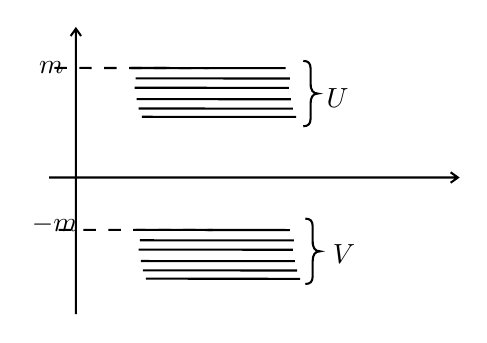
\begin{tikzpicture}[x=0.75pt,y=0.75pt,yscale=-0.5,xscale=0.5]
%uncomment if require: \path (0,300); %set diagram left start at 0, and has height of 300

%Shape: Axis 2D [id:dp3983214191540887] 
\draw  (125.57,154.54) -- (519.57,154.54)(151.46,11.14) -- (151.46,286.14) (512.57,149.54) -- (519.57,154.54) -- (512.57,159.54) (146.46,18.14) -- (151.46,11.14) -- (156.46,18.14)  ;
%Straight Lines [id:da031448643395316056] 
\draw    (205,49) -- (353.57,49.14) ;
%Straight Lines [id:da9959233359352435] 
\draw    (209,59) -- (357.57,59.14) ;
%Straight Lines [id:da5841252618565393] 
\draw    (208,68) -- (356.57,68.14) ;
%Straight Lines [id:da27134091658819925] 
\draw    (210,79) -- (358.57,79.14) ;
%Straight Lines [id:da18838152782543283] 
\draw    (212,88) -- (360.57,88.14) ;
%Straight Lines [id:da7760563463183436] 
\draw    (215,96) -- (363.57,96.14) ;
%Straight Lines [id:da4455262039617256] 
\draw    (209,205) -- (357.57,205.14) ;
%Straight Lines [id:da10206692557234542] 
\draw    (213,215) -- (361.57,215.14) ;
%Straight Lines [id:da0799601657045017] 
\draw    (212,224) -- (360.57,224.14) ;
%Straight Lines [id:da21576180746597706] 
\draw    (214,235) -- (362.57,235.14) ;
%Straight Lines [id:da6749140692469682] 
\draw    (216,244) -- (364.57,244.14) ;
%Straight Lines [id:da7415268598996998] 
\draw    (219,252) -- (367.57,252.14) ;
%Shape: Brace [id:dp23943847238752913] 
\draw   (370.57,105.14) .. controls (375.24,105.14) and (377.57,102.81) .. (377.57,98.14) -- (377.57,83.64) .. controls (377.57,76.97) and (379.9,73.64) .. (384.57,73.64) .. controls (379.9,73.64) and (377.57,70.31) .. (377.57,63.64)(377.57,66.64) -- (377.57,49.14) .. controls (377.57,44.47) and (375.24,42.14) .. (370.57,42.14) ;
%Shape: Brace [id:dp5196707362747854] 
\draw   (372.57,257.14) .. controls (377.24,257.14) and (379.57,254.81) .. (379.57,250.14) -- (379.57,235.64) .. controls (379.57,228.97) and (381.9,225.64) .. (386.57,225.64) .. controls (381.9,225.64) and (379.57,222.31) .. (379.57,215.64)(379.57,218.64) -- (379.57,201.14) .. controls (379.57,196.47) and (377.24,194.14) .. (372.57,194.14) ;
%Straight Lines [id:da9743373505676289] 
\draw  [dash pattern={on 4.5pt off 4.5pt}]  (134.71,204.93) -- (283.29,205.07) ;
%Straight Lines [id:da68540932096566] 
\draw  [dash pattern={on 4.5pt off 4.5pt}]  (130.71,48.93) -- (279.29,49.07) ;

% Text Node
\draw (113,39.4) node [anchor=north west][inner sep=0.75pt]    {$m$};
% Text Node
\draw (106,188.4) node [anchor=north west][inner sep=0.75pt]    {$-m$};
% Text Node
\draw (390,65.4) node [anchor=north west][inner sep=0.75pt]    {$U$};
% Text Node
\draw (396,216.4) node [anchor=north west][inner sep=0.75pt]    {$V$};


\end{tikzpicture}
  \caption[Mar de Dirac]{Soluciones de la ecuación de Dirac}
  \label{fig:MD}
\end{marginfigure}

Dirac propuso lo que se conce como el mar de Dirac
\begin{definition}[Mar de Dirac]
  El mar de Dirac propone que todos los niveles con energía negativa estan llenos (u ocupados) por estados, dado que Dirac trabajaba con fermiones hay que tener en cuenta el principio de exclusión de Pauli y por lo tanto hay un número fínito de electrones que pueden ocupar dichos estados.

  Esto quiere decir que el vacio no está realmente vacio, si no que esta lleno, tan lleno que no cabe nada más y por lo tanto no son estados accesibles. Lo que se puede interpretar como que ese es el estado fundamental. 
\end{definition}

En este caso Dirac tuvo suerte, ya que al tratar con fermiones se saco el principio de exclusión de Pauli como un as bajo la manga, pero con los bosones ese truco no funciona. 

Ahora veamos como llegamos de eso a la exsitencia de antipartículas con toda la magía que conlleva. Las antípartículas nacen de esta interpretación por las excitaciones del vacio mediantes campos electromagnéticos (Ver figura \ref{fig:Antipartículas}) las cuales hacen saltar a los estados con masa negativas a masas positivas (más o menos como los huecos que contaban en estado sólido). 

\begin{marginfigure}[]


  \tikzset{every picture/.style={line width=0.75pt}} %set default line width to 0.75pt        

  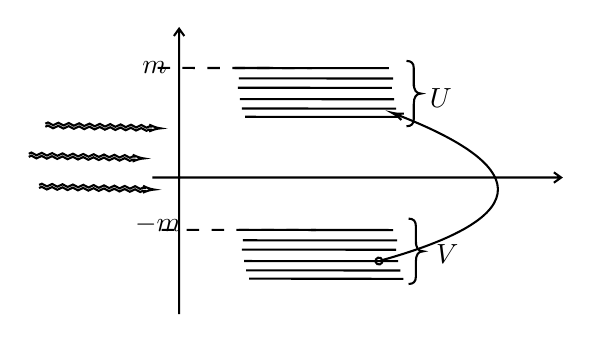
\begin{tikzpicture}[x=0.75pt,y=0.75pt,yscale=-0.5,xscale=0.5]
  %uncomment if require: \path (0,300); %set diagram left start at 0, and has height of 300
  
  %Shape: Axis 2D [id:dp3983214191540887] 
  \draw  (125.57,154.54) -- (519.57,154.54)(151.46,11.14) -- (151.46,286.14) (512.57,149.54) -- (519.57,154.54) -- (512.57,159.54) (146.46,18.14) -- (151.46,11.14) -- (156.46,18.14)  ;
  %Straight Lines [id:da031448643395316056] 
  \draw    (205,49) -- (353.57,49.14) ;
  %Straight Lines [id:da9959233359352435] 
  \draw    (209,59) -- (357.57,59.14) ;
  %Straight Lines [id:da5841252618565393] 
  \draw    (208,68) -- (356.57,68.14) ;
  %Straight Lines [id:da27134091658819925] 
  \draw    (210,79) -- (358.57,79.14) ;
  %Straight Lines [id:da18838152782543283] 
  \draw    (212,88) -- (360.57,88.14) ;
  %Straight Lines [id:da7760563463183436] 
  \draw    (215,96) -- (363.57,96.14) ;
  %Straight Lines [id:da4455262039617256] 
  \draw    (209,205) -- (357.57,205.14) ;
  %Straight Lines [id:da10206692557234542] 
  \draw    (213,215) -- (361.57,215.14) ;
  %Straight Lines [id:da0799601657045017] 
  \draw    (212,224) -- (360.57,224.14) ;
  %Straight Lines [id:da21576180746597706] 
  \draw    (214,235) -- (362.57,235.14) ;
  %Straight Lines [id:da6749140692469682] 
  \draw    (216,244) -- (364.57,244.14) ;
  %Straight Lines [id:da7415268598996998] 
  \draw    (219,252) -- (367.57,252.14) ;
  %Shape: Brace [id:dp23943847238752913] 
  \draw   (370.57,105.14) .. controls (375.24,105.14) and (377.57,102.81) .. (377.57,98.14) -- (377.57,83.64) .. controls (377.57,76.97) and (379.9,73.64) .. (384.57,73.64) .. controls (379.9,73.64) and (377.57,70.31) .. (377.57,63.64)(377.57,66.64) -- (377.57,49.14) .. controls (377.57,44.47) and (375.24,42.14) .. (370.57,42.14) ;
  %Shape: Brace [id:dp5196707362747854] 
  \draw   (372.57,257.14) .. controls (377.24,257.14) and (379.57,254.81) .. (379.57,250.14) -- (379.57,235.64) .. controls (379.57,228.97) and (381.9,225.64) .. (386.57,225.64) .. controls (381.9,225.64) and (379.57,222.31) .. (379.57,215.64)(379.57,218.64) -- (379.57,201.14) .. controls (379.57,196.47) and (377.24,194.14) .. (372.57,194.14) ;
  %Straight Lines [id:da9743373505676289] 
  \draw  [dash pattern={on 4.5pt off 4.5pt}]  (134.71,204.93) -- (283.29,205.07) ;
  %Straight Lines [id:da68540932096566] 
  \draw  [dash pattern={on 4.5pt off 4.5pt}]  (130.71,48.93) -- (279.29,49.07) ;
  %Curve Lines [id:da8414489739291839] 
  \draw    (346.63,234.27) .. controls (519.17,185.87) and (467.54,134.45) .. (358.22,92.77) ;
  \draw [shift={(356.57,92.14)}, rotate = 20.73] [color={rgb, 255:red, 0; green, 0; blue, 0 }  ][line width=0.75]    (10.93,-3.29) .. controls (6.95,-1.4) and (3.31,-0.3) .. (0,0) .. controls (3.31,0.3) and (6.95,1.4) .. (10.93,3.29)   ;
  \draw [shift={(344,235)}, rotate = 344.53] [color={rgb, 255:red, 0; green, 0; blue, 0 }  ][line width=0.75]      (0, 0) circle [x radius= 3.35, y radius= 3.35]   ;
  %Straight Lines [id:da44668845645125677] 
  \draw    (22.61,102.64) .. controls (24.32,101.02) and (25.99,101.07) .. (27.61,102.78) .. controls (29.24,104.49) and (30.9,104.53) .. (32.61,102.91) .. controls (34.32,101.29) and (35.99,101.34) .. (37.61,103.05) .. controls (39.23,104.76) and (40.89,104.8) .. (42.6,103.18) .. controls (44.31,101.56) and (45.98,101.61) .. (47.6,103.32) .. controls (49.23,105.03) and (50.89,105.07) .. (52.6,103.45) .. controls (54.31,101.83) and (55.98,101.88) .. (57.6,103.59) .. controls (59.23,105.3) and (60.89,105.34) .. (62.6,103.72) .. controls (64.31,102.1) and (65.98,102.15) .. (67.6,103.86) .. controls (69.22,105.57) and (70.88,105.61) .. (72.59,103.99) .. controls (74.3,102.37) and (75.97,102.42) .. (77.59,104.13) .. controls (79.22,105.84) and (80.88,105.88) .. (82.59,104.26) .. controls (84.3,102.64) and (85.97,102.69) .. (87.59,104.4) .. controls (89.22,106.11) and (90.88,106.15) .. (92.59,104.53) .. controls (94.3,102.91) and (95.97,102.96) .. (97.58,104.67) .. controls (99.21,106.38) and (100.87,106.42) .. (102.58,104.8) .. controls (104.29,103.18) and (105.96,103.23) .. (107.58,104.94) .. controls (109.21,106.65) and (110.87,106.69) .. (112.58,105.07) .. controls (114.29,103.45) and (115.96,103.5) .. (117.58,105.21) .. controls (119.2,106.92) and (120.87,106.97) .. (122.58,105.35) -- (122.62,105.35) -- (125.61,105.43)(22.53,105.64) .. controls (24.24,104.02) and (25.91,104.07) .. (27.53,105.78) .. controls (29.16,107.49) and (30.82,107.53) .. (32.53,105.91) .. controls (34.24,104.29) and (35.91,104.34) .. (37.53,106.05) .. controls (39.15,107.76) and (40.81,107.8) .. (42.52,106.18) .. controls (44.23,104.56) and (45.9,104.61) .. (47.52,106.32) .. controls (49.15,108.03) and (50.81,108.07) .. (52.52,106.45) .. controls (54.23,104.83) and (55.9,104.88) .. (57.52,106.59) .. controls (59.15,108.3) and (60.81,108.34) .. (62.52,106.72) .. controls (64.23,105.1) and (65.9,105.15) .. (67.51,106.86) .. controls (69.14,108.57) and (70.8,108.61) .. (72.51,106.99) .. controls (74.22,105.37) and (75.89,105.42) .. (77.51,107.13) .. controls (79.14,108.84) and (80.8,108.88) .. (82.51,107.26) .. controls (84.22,105.64) and (85.89,105.69) .. (87.51,107.4) .. controls (89.14,109.11) and (90.8,109.15) .. (92.51,107.53) .. controls (94.22,105.91) and (95.89,105.96) .. (97.5,107.67) .. controls (99.13,109.38) and (100.79,109.42) .. (102.5,107.8) .. controls (104.21,106.18) and (105.88,106.23) .. (107.5,107.94) .. controls (109.13,109.65) and (110.79,109.69) .. (112.5,108.07) .. controls (114.21,106.45) and (115.88,106.5) .. (117.5,108.21) .. controls (119.12,109.92) and (120.78,109.96) .. (122.49,108.34) -- (122.53,108.35) -- (125.53,108.43) ;
  \draw [shift={(133.57,107.14)}, rotate = 181.55] [color={rgb, 255:red, 0; green, 0; blue, 0 }  ][line width=0.75]    (10.93,-3.29) .. controls (6.95,-1.4) and (3.31,-0.3) .. (0,0) .. controls (3.31,0.3) and (6.95,1.4) .. (10.93,3.29)   ;
  %Straight Lines [id:da23159056240315867] 
  \draw    (6.61,131.64) .. controls (8.32,130.02) and (9.99,130.07) .. (11.61,131.78) .. controls (13.24,133.49) and (14.9,133.53) .. (16.61,131.91) .. controls (18.32,130.29) and (19.99,130.34) .. (21.61,132.05) .. controls (23.23,133.76) and (24.89,133.8) .. (26.6,132.18) .. controls (28.31,130.56) and (29.98,130.61) .. (31.6,132.32) .. controls (33.23,134.03) and (34.89,134.07) .. (36.6,132.45) .. controls (38.31,130.83) and (39.98,130.88) .. (41.6,132.59) .. controls (43.23,134.3) and (44.89,134.34) .. (46.6,132.72) .. controls (48.31,131.1) and (49.98,131.15) .. (51.6,132.86) .. controls (53.22,134.57) and (54.88,134.61) .. (56.59,132.99) .. controls (58.3,131.37) and (59.97,131.42) .. (61.59,133.13) .. controls (63.22,134.84) and (64.88,134.88) .. (66.59,133.26) .. controls (68.3,131.64) and (69.97,131.69) .. (71.59,133.4) .. controls (73.22,135.11) and (74.88,135.15) .. (76.59,133.53) .. controls (78.3,131.91) and (79.97,131.96) .. (81.58,133.67) .. controls (83.21,135.38) and (84.87,135.42) .. (86.58,133.8) .. controls (88.29,132.18) and (89.96,132.23) .. (91.58,133.94) .. controls (93.21,135.65) and (94.87,135.69) .. (96.58,134.07) .. controls (98.29,132.45) and (99.96,132.5) .. (101.58,134.21) .. controls (103.2,135.92) and (104.87,135.97) .. (106.58,134.35) -- (106.62,134.35) -- (109.61,134.43)(6.53,134.64) .. controls (8.24,133.02) and (9.91,133.07) .. (11.53,134.78) .. controls (13.16,136.49) and (14.82,136.53) .. (16.53,134.91) .. controls (18.24,133.29) and (19.91,133.34) .. (21.53,135.05) .. controls (23.15,136.76) and (24.81,136.8) .. (26.52,135.18) .. controls (28.23,133.56) and (29.9,133.61) .. (31.52,135.32) .. controls (33.15,137.03) and (34.81,137.07) .. (36.52,135.45) .. controls (38.23,133.83) and (39.9,133.88) .. (41.52,135.59) .. controls (43.15,137.3) and (44.81,137.34) .. (46.52,135.72) .. controls (48.23,134.1) and (49.9,134.15) .. (51.51,135.86) .. controls (53.14,137.57) and (54.8,137.61) .. (56.51,135.99) .. controls (58.22,134.37) and (59.89,134.42) .. (61.51,136.13) .. controls (63.14,137.84) and (64.8,137.88) .. (66.51,136.26) .. controls (68.22,134.64) and (69.89,134.69) .. (71.51,136.4) .. controls (73.14,138.11) and (74.8,138.15) .. (76.51,136.53) .. controls (78.22,134.91) and (79.89,134.96) .. (81.5,136.67) .. controls (83.13,138.38) and (84.79,138.42) .. (86.5,136.8) .. controls (88.21,135.18) and (89.88,135.23) .. (91.5,136.94) .. controls (93.13,138.65) and (94.79,138.69) .. (96.5,137.07) .. controls (98.21,135.45) and (99.88,135.5) .. (101.5,137.21) .. controls (103.12,138.92) and (104.78,138.96) .. (106.49,137.34) -- (106.53,137.35) -- (109.53,137.43) ;
  \draw [shift={(117.57,136.14)}, rotate = 181.55] [color={rgb, 255:red, 0; green, 0; blue, 0 }  ][line width=0.75]    (10.93,-3.29) .. controls (6.95,-1.4) and (3.31,-0.3) .. (0,0) .. controls (3.31,0.3) and (6.95,1.4) .. (10.93,3.29)   ;
  %Straight Lines [id:da4339308463725169] 
  \draw    (16.61,161.64) .. controls (18.32,160.02) and (19.99,160.07) .. (21.61,161.78) .. controls (23.24,163.49) and (24.9,163.53) .. (26.61,161.91) .. controls (28.32,160.29) and (29.99,160.34) .. (31.61,162.05) .. controls (33.23,163.76) and (34.89,163.8) .. (36.6,162.18) .. controls (38.31,160.56) and (39.98,160.61) .. (41.6,162.32) .. controls (43.23,164.03) and (44.89,164.07) .. (46.6,162.45) .. controls (48.31,160.83) and (49.98,160.88) .. (51.6,162.59) .. controls (53.23,164.3) and (54.89,164.34) .. (56.6,162.72) .. controls (58.31,161.1) and (59.98,161.15) .. (61.6,162.86) .. controls (63.22,164.57) and (64.88,164.61) .. (66.59,162.99) .. controls (68.3,161.37) and (69.97,161.42) .. (71.59,163.13) .. controls (73.22,164.84) and (74.88,164.88) .. (76.59,163.26) .. controls (78.3,161.64) and (79.97,161.69) .. (81.59,163.4) .. controls (83.22,165.11) and (84.88,165.15) .. (86.59,163.53) .. controls (88.3,161.91) and (89.97,161.96) .. (91.58,163.67) .. controls (93.21,165.38) and (94.87,165.42) .. (96.58,163.8) .. controls (98.29,162.18) and (99.96,162.23) .. (101.58,163.94) .. controls (103.21,165.65) and (104.87,165.69) .. (106.58,164.07) .. controls (108.29,162.45) and (109.96,162.5) .. (111.58,164.21) .. controls (113.2,165.92) and (114.87,165.97) .. (116.58,164.35) -- (116.62,164.35) -- (119.61,164.43)(16.53,164.64) .. controls (18.24,163.02) and (19.91,163.07) .. (21.53,164.78) .. controls (23.16,166.49) and (24.82,166.53) .. (26.53,164.91) .. controls (28.24,163.29) and (29.91,163.34) .. (31.53,165.05) .. controls (33.15,166.76) and (34.81,166.8) .. (36.52,165.18) .. controls (38.23,163.56) and (39.9,163.61) .. (41.52,165.32) .. controls (43.15,167.03) and (44.81,167.07) .. (46.52,165.45) .. controls (48.23,163.83) and (49.9,163.88) .. (51.52,165.59) .. controls (53.15,167.3) and (54.81,167.34) .. (56.52,165.72) .. controls (58.23,164.1) and (59.9,164.15) .. (61.51,165.86) .. controls (63.14,167.57) and (64.8,167.61) .. (66.51,165.99) .. controls (68.22,164.37) and (69.89,164.42) .. (71.51,166.13) .. controls (73.14,167.84) and (74.8,167.88) .. (76.51,166.26) .. controls (78.22,164.64) and (79.89,164.69) .. (81.51,166.4) .. controls (83.14,168.11) and (84.8,168.15) .. (86.51,166.53) .. controls (88.22,164.91) and (89.89,164.96) .. (91.5,166.67) .. controls (93.13,168.38) and (94.79,168.42) .. (96.5,166.8) .. controls (98.21,165.18) and (99.88,165.23) .. (101.5,166.94) .. controls (103.13,168.65) and (104.79,168.69) .. (106.5,167.07) .. controls (108.21,165.45) and (109.88,165.5) .. (111.5,167.21) .. controls (113.12,168.92) and (114.78,168.96) .. (116.49,167.34) -- (116.53,167.35) -- (119.53,167.43) ;
  \draw [shift={(127.57,166.14)}, rotate = 181.55] [color={rgb, 255:red, 0; green, 0; blue, 0 }  ][line width=0.75]    (10.93,-3.29) .. controls (6.95,-1.4) and (3.31,-0.3) .. (0,0) .. controls (3.31,0.3) and (6.95,1.4) .. (10.93,3.29)   ;
  
  % Text Node
  \draw (113,39.4) node [anchor=north west][inner sep=0.75pt]    {$m$};
  % Text Node
  \draw (106,188.4) node [anchor=north west][inner sep=0.75pt]    {$-m$};
  % Text Node
  \draw (390,65.4) node [anchor=north west][inner sep=0.75pt]    {$U$};
  % Text Node
  \draw (396,216.4) node [anchor=north west][inner sep=0.75pt]    {$V$};
  
  
  \end{tikzpicture}
  
  \caption[Antipartículas]{Excitación del mar de Dirac por un campo electromagnético}
  \label{fig:Antipartículas}
\end{marginfigure}

Por razones que no apunté o Dobado no contó, al parecer estos huecos como pasan a tener ahora masa posotiva pero su energía (o algo, estoy inventando un poco) se conserva, estas deben tener carga contraria (en carga inserte propiedad cualquiera). 
\section{Fermiones quirales}

A continuación definimos la matriz $\gamma^5$ en la representación de Weyl, que será la que usemos de ahora en adelante para este curso.

\begin{DispWithArrows}[format=c, displaystyle]
  \gamma^5= i\gamma^0\gamma^1\gamma^2\gamma^3= \begin{bmatrix}
      -1 & 0 \\
      0 & 1
  \end{bmatrix}
  \label{eq:}
\end{DispWithArrows}

Algunas propiedades de $\gamma^5$ son:
\begin{itemize}
  \item $\gamma^5=(\gamma^5)^\dagger$
  \item $\gamma^\mu\gamma^5=-\gamma^5\gamma^\mu$
  \item $\acom{\gamma^\mu}{\gamma^5}=$
  \item $(\gamma^5)^2= \mathcal{I}$
\end{itemize}

\subsection{Proyectores de Weyl}

A continuación definiremos los proyectores Weyl y posteriormente los formularemos.

\begin{definition}[Proyectores Weyl]
  Los proyectroes Weyl son unos operadores que nos devuelven el espinor de Weyl correspondiente, esto es, $\psi_{L}$ o $\phi_{R}$ una vez aplicados a la función de onda. 
  Estos operadores se definen como:

  $$
P_{L}=\frac{1}{2}\left(1-\gamma^{5}\right)=\left(\begin{array}{ll}
\mathbb{1} & 0 \\
0 & 0
\end{array}\right) \quad P_{R}=\frac{1}{2}\left(1+\gamma^{5}\right)=\left(\begin{array}{ll}
0 & 0 \\
0 & \mathbb{1}
\end{array}\right)
$$
\end{definition}

Estos operadores tienen las siguientes propiedades:
\begin{itemize}
  \item $P_{L}^{2}=P_{L}$ y $P_{R}^{2}=P_{R}$
  \item $P_{L} P_{R}=P_{R} P_{L}=0$
  \item $P_{L}+P_{R}=\mathbb{1}$
  \item $\gamma_{\mu} P_{L}=P_{R} \gamma^{\mu}$
\end{itemize}

Podemos escribir el cuadriespinor en terminos de estos operadores, que nos lo dividen en su componente levógira y dextrógira, respectivamente:
$$
\psi=\binom{\varepsilon}{\chi} \rightarrow \psi=\psi_{L}+\psi_{R}=P_{L} \psi+P_{R} \psi=\binom{\varepsilon}{0}+\binom{0}{\chi}
$$

Si introducimos ahora estos operadores en la ecuación de Dirac:
$$
(i \not \partial-m) \psi=0 \rightarrow\left\{\begin{array}{l}
i \not \psi_{R}=m \psi_{L} \\
i \not \psi_{L}=m \psi_{R}
\end{array}\right.
$$

Se demostró que las partículas con masa nula no tienen parte dextrógira y se pueden describir únicamente con la parte levógira. En representación de Weyl:
$$
\left.\begin{array}{l}
\text { Levógiro: }\left(\frac{1}{2}, 0\right) \\
\text { Dextrógiro: }\left(0, \frac{1}{2}\right)
\end{array}\right\} \text { Fermiones de Dirac: } \psi_{D}=\overbrace{\left(\frac{1}{2}, 0\right)}^{\psi_{L} \sim \varepsilon} \oplus \overbrace{\left(0, \frac{1}{2}\right)}^{\psi_{R} \sim \chi}
$$

